\documentclass[tikz,border=0.5cm]{standalone}
\usetikzlibrary{decorations.pathreplacing}
\begin{document}
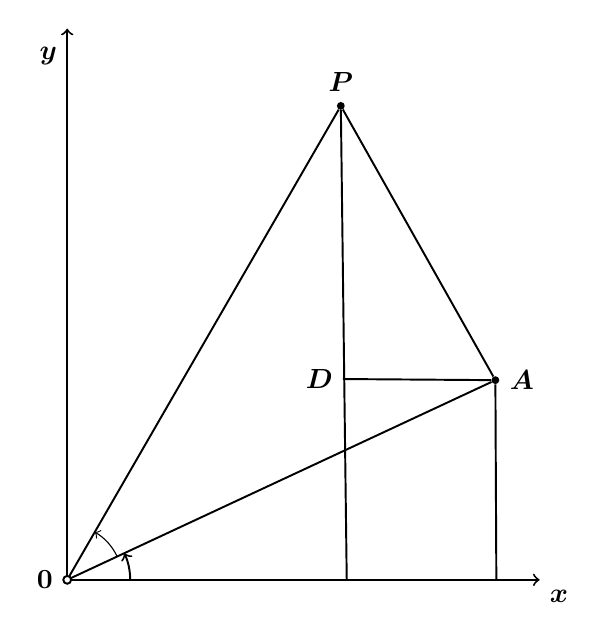
\begin{tikzpicture}[font=\boldmath, decoration = {brace,raise=4pt},line width=0.7pt]
\foreach \n/\s/\l/\p/\a in {o/draw/{$0$}/{0,0}/left,A/fill/{$A$}/{25:6}/right,P/fill/{$P$}/{60:6.95}/above}
    \node (\n)[\s,circle,scale=0.3,label={\a:\l}]at (\p){};
\draw (o) [->] edge (6,0)
      [-] edge (A)
      [-] edge (P);
\draw (6,0) node[anchor=north west] {$x$};
\draw (o) [->] edge (0,7);
\draw (A)  edge (P);
\draw (0,6.9) node[anchor=north east] {$y$};
\draw (3.5,2.8) node[anchor=north east] {$D$};
\draw (5.45,0) [-] edge (A);
\draw (3.55,0) [-] edge (P);
\draw (A) [-] edge (3.5,2.55);
\foreach \t/\a/\b/\r in {/0/25/0.8,thin/25/60/0.7}
    \draw [->,\t](\a:\r) arc (\a:\b:\r);
\end{tikzpicture}
\end{document} 